%%%%%%%%%%%%%%%%%%%%%%%%%%%%%%%%%%%%%%%%%%%%%%%%%%%%%%%%
% IE643 Course Project Poster -- Gradient Mavericks
% Built from the official "IE643 2026 Course Project Poster Sample" (a0poster, portrait).
% Header layout, colours, frame, section order kept; content filled in.
% Build: ~/miniconda3/envs/tex/bin/tectonic Gradient_Mavericks_IE643_Poster.tex
%%%%%%%%%%%%%%%%%%%%%%%%%%%%%%%%%%%%%%%%%%%%%%%%%%%%%%%%
\documentclass[a0,portrait]{a0poster}
\usepackage[top=5cm, bottom=0.3cm, left=5cm, right=3cm]{geometry}
\usepackage[compact]{titlesec}
\usepackage{multicol}
\columnsep=100pt
\columnseprule=15pt
\usepackage[svgnames]{xcolor}
\usepackage{palatino}
\usepackage{xkeyval}
\usepackage{graphicx}
\setlength{\abovecaptionskip}{5pt plus 5pt minus 3pt}
\graphicspath{{figures/}{figs/}}
\usepackage{booktabs}
\usepackage[font=small,labelfont=bf]{caption}
\usepackage{amsfonts, amsmath, amsthm, amssymb}
\usepackage{csquotes}
\usepackage{wrapfig}
\usepackage{multirow}
\usepackage{makecell}
\def\columnseprulecolor{\color{NavyBlue}}%
\usepackage{framed}
\colorlet{frameborder}{NavyBlue}
\usepackage{tikz}
\usetikzlibrary{arrows.meta,positioning,calc}
\usepackage{enumitem}
\setlist[itemize]{leftmargin=1.3em, itemsep=4pt, topsep=4pt}

\newcommand{\z}{\mathbf{z}}
\newcommand{\hx}{\hat{\mathbf{x}}_0}
\newcommand{\todo}[1]{\textcolor{red}{#1}}

\begin{document}
\begin{minipage}[c]{\linewidth}
\vspace{0.1cm}
\noindent\makebox[\textwidth][c]{
\begin{minipage}[c]{0.14\linewidth}
\vspace{0pt}\raggedright
\hspace{1cm}

\includegraphics[scale=1.3,width=\linewidth]{figures/logo.png}
\end{minipage}
\hfill
\begin{minipage}[c]{0.75\textwidth}
\centering
\Huge \color{Green} \textbf{IE643 Course Project}\\[0.5cm]
\Huge \color{NavyBlue} \textbf{Text-Conditioned Synthetic Chest X-ray Generation}\\[0.2cm]
\Huge \color{NavyBlue} \textbf{Using Diffusion Models for Data Augmentation}\\[0.5cm]
\Large \color{NavyBlue} \textbf{Team: Gradient Mavericks}\\[0.5cm]
\large \color{Black} \textbf{Saksham Jain $^{1}$ (\todo{Roll Number}), Somya Dahiaya $^{2}$ (\todo{Roll Number})}\\[0.2cm]
\small \text{\todo{XXXX@iitb.ac.in}$^{1}$, \todo{XXXXX@iitb.ac.in}$^{2}$}\\
\large \color{Green} \textbf{}\\
\end{minipage}
\begin{minipage}[c]{0.145\textwidth}
\vspace{0pt}\raggedleft

\includegraphics[scale=1.3,width=\linewidth]{figures/IE643-Logo.pdf}
\hspace{1cm}
\end{minipage}}
\\[0.1cm]%
\color{NavyBlue}\setlength\FrameRule{25pt}
\begin{framed}
\vspace{0.5cm}
\begin{multicols}{2}
%----------------------------------------------------------------------------------------
%	Abstract
%----------------------------------------------------------------------------------------
\color{Black}
\small
\section*{Abstract}
We LoRA-fine-tune a Stable Diffusion~1.5 chest X-ray (CXR) generator for rare findings and add a \textbf{frozen-classifier loss} (``shows the requested finding'') and an \textbf{adversarial loss} (``looks real'') to the denoising loss. Judged by held-out models, the requested-finding rate rises \textbf{15.7\%$\to$51.2\%} and defects fall \textbf{32.7\%$\to$18.2\%}. A DenseNet-121 trained on real + synthetic images reaches parity with real-only (0.283 vs.\ 0.285 macro-F1) but does not beat it, as prior work predicts for full-data settings.

%----------------------------------------------------------------------------------------
%	INTRODUCTION
%----------------------------------------------------------------------------------------
\section*{Introduction}
\begin{itemize}
	\item Rare CheXpert findings (\textbf{Pleural Other, Pneumonia, Lung Lesion, Enl.\ Cardiomediastinum, Fracture}) have only 241--1{,}327 clean images; text-to-image diffusion~[1,2] could rebalance them.
	\item Failure modes: the generator \textbf{ignores the prompt} or makes \textbf{implausible anatomy}; the denoising loss measures neither.
\end{itemize}
We outline our major \textbf{contributions} below:
\begin{itemize}
	\item \textbf{Frozen-classifier (CE) + conditional adversarial losses} in LoRA fine-tuning, on a differentiable one-step image estimate (ReFL-style~[3]).
	\item CE alone \textbf{reward-hacks} (78.5\% defects); a bounded \textbf{matched-confidence margin loss} fixes it.
	\item \textbf{Held-out judges} for per-pathology finding / defect rates and checkpoint selection; leakage-free downstream protocol, \textbf{19 settings $\times$ 3 seeds}.
\end{itemize}

%----------------------------------------------------------------------------------------
%	Workflow
%----------------------------------------------------------------------------------------
\section*{Workflow}
\begin{center}
\resizebox{0.8\linewidth}{!}{%
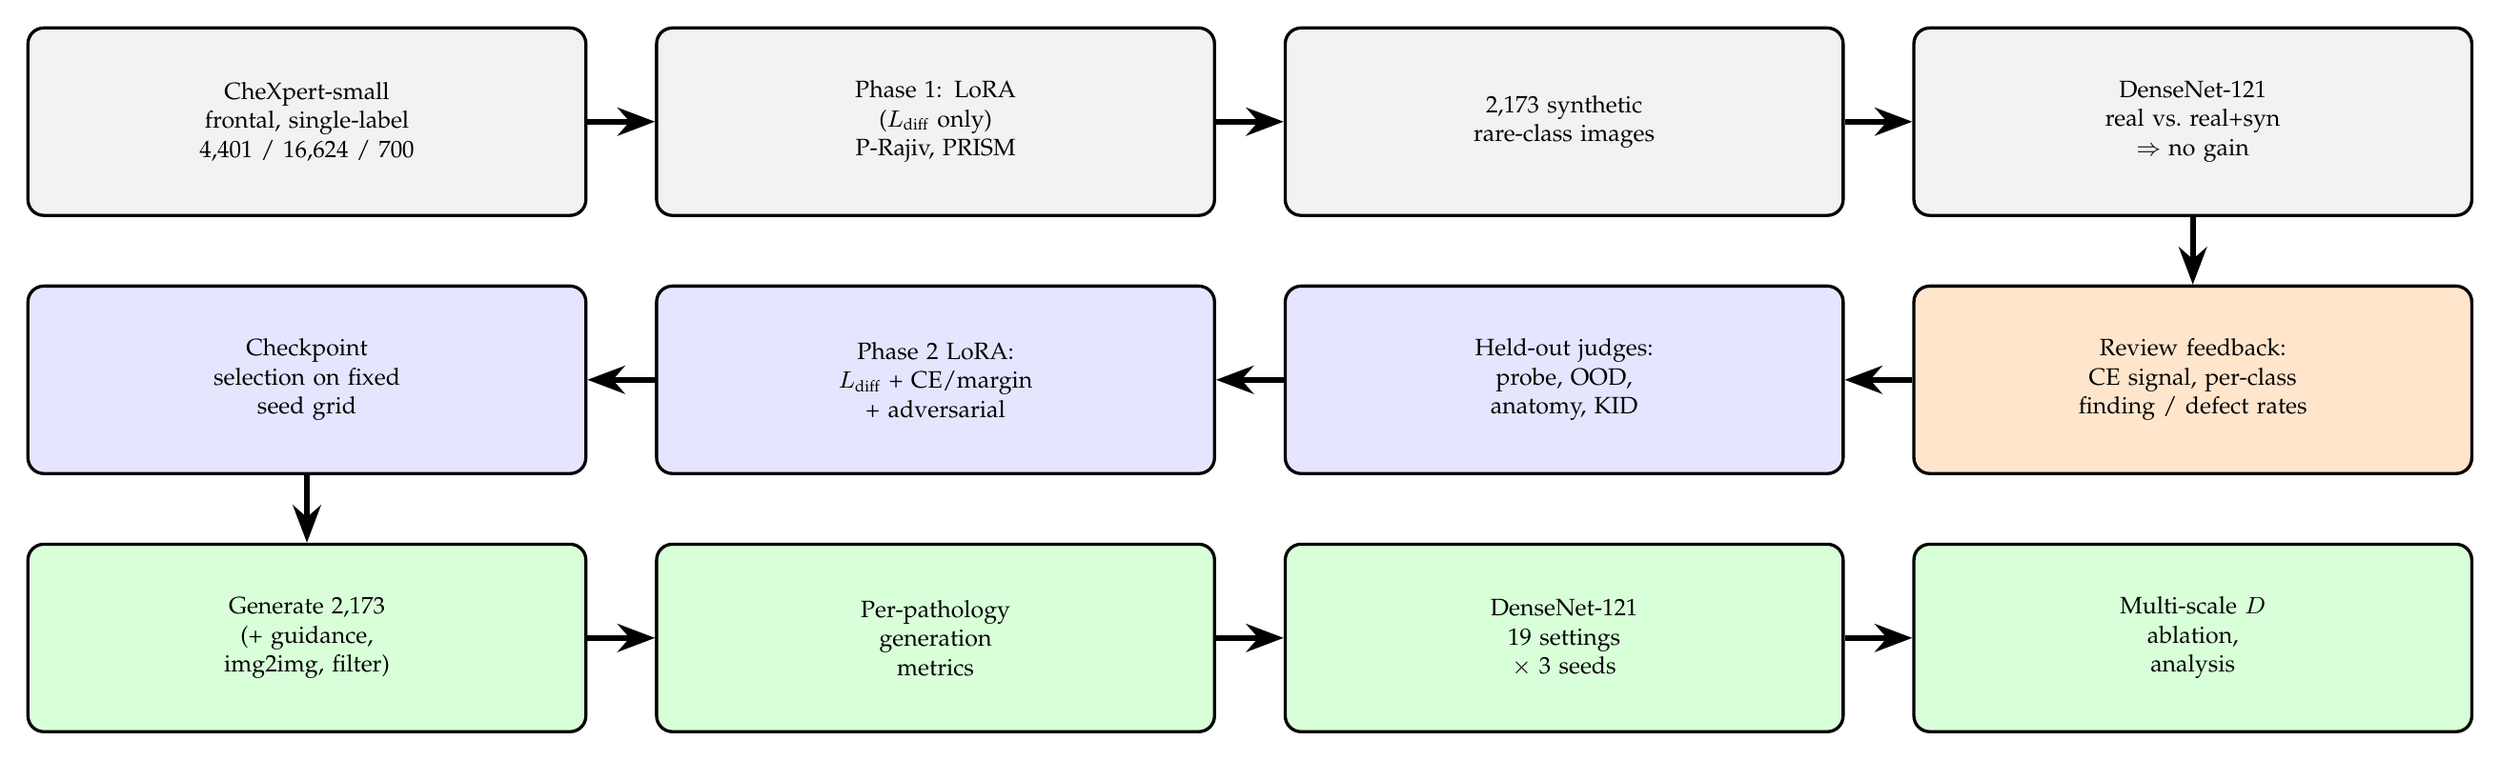
\begin{tikzpicture}[
  node distance=7mm and 9mm,
  box/.style={draw, very thick, rounded corners=6pt, align=center, font=\small, minimum height=2.5cm, text width=7.2cm, fill=#1},
  box/.default=white,
  arr/.style={-{Stealth[length=5mm]}, line width=2pt}]
\node[box=gray!10] (data) {CheXpert-small\\frontal, single-label\\4{,}401 / 16{,}624 / 700};
\node[box=gray!10, right=of data] (p1) {Phase 1: LoRA\\($L_{\text{diff}}$ only)\\P-Rajiv, PRISM};
\node[box=gray!10, right=of p1] (g1) {2{,}173 synthetic\\rare-class images};
\node[box=gray!10, right=of g1] (c1) {DenseNet-121\\real vs.\ real+syn\\$\Rightarrow$ no gain};
\node[box=orange!20, below=9mm of c1] (fb) {Review feedback:\\CE signal, per-class\\finding / defect rates};
\node[box=blue!10, left=of fb] (judge) {Held-out judges:\\probe, OOD,\\anatomy, KID};
\node[box=blue!10, left=of judge] (p2) {Phase 2 LoRA:\\$L_{\text{diff}}$ + CE/margin\\+ adversarial};
\node[box=blue!10, left=of p2] (sel) {Checkpoint\\selection on fixed\\seed grid};
\node[box=green!15, below=9mm of sel] (gen) {Generate 2{,}173\\(+ guidance,\\img2img, filter)};
\node[box=green!15, right=of gen] (eval) {Per-pathology\\generation\\metrics};
\node[box=green!15, right=of eval] (ds) {DenseNet-121\\19 settings\\$\times$ 3 seeds};
\node[box=green!15, right=of ds] (rep) {Multi-scale $D$\\ablation,\\analysis};
\draw[arr] (data)--(p1); \draw[arr] (p1)--(g1); \draw[arr] (g1)--(c1); \draw[arr] (c1)--(fb);
\draw[arr] (fb)--(judge); \draw[arr] (judge)--(p2); \draw[arr] (p2)--(sel); \draw[arr] (sel)--(gen);
\draw[arr] (gen)--(eval); \draw[arr] (eval)--(ds); \draw[arr] (ds)--(rep);
\end{tikzpicture}}
\captionof{figure}{\color{Blue} Overall workflow. Grey: phase 1; orange: review feedback; blue/green: novelty phase.}
\label{workflow}
\end{center}

%----------------------------------------------------------------------------------------
%	Methodology
%----------------------------------------------------------------------------------------
\section*{Methodology}
All runs continue from the phase-1 P-Rajiv LoRA (rank 16, UNet attention + text encoder).
\begin{center}
\resizebox{0.88\linewidth}{!}{%
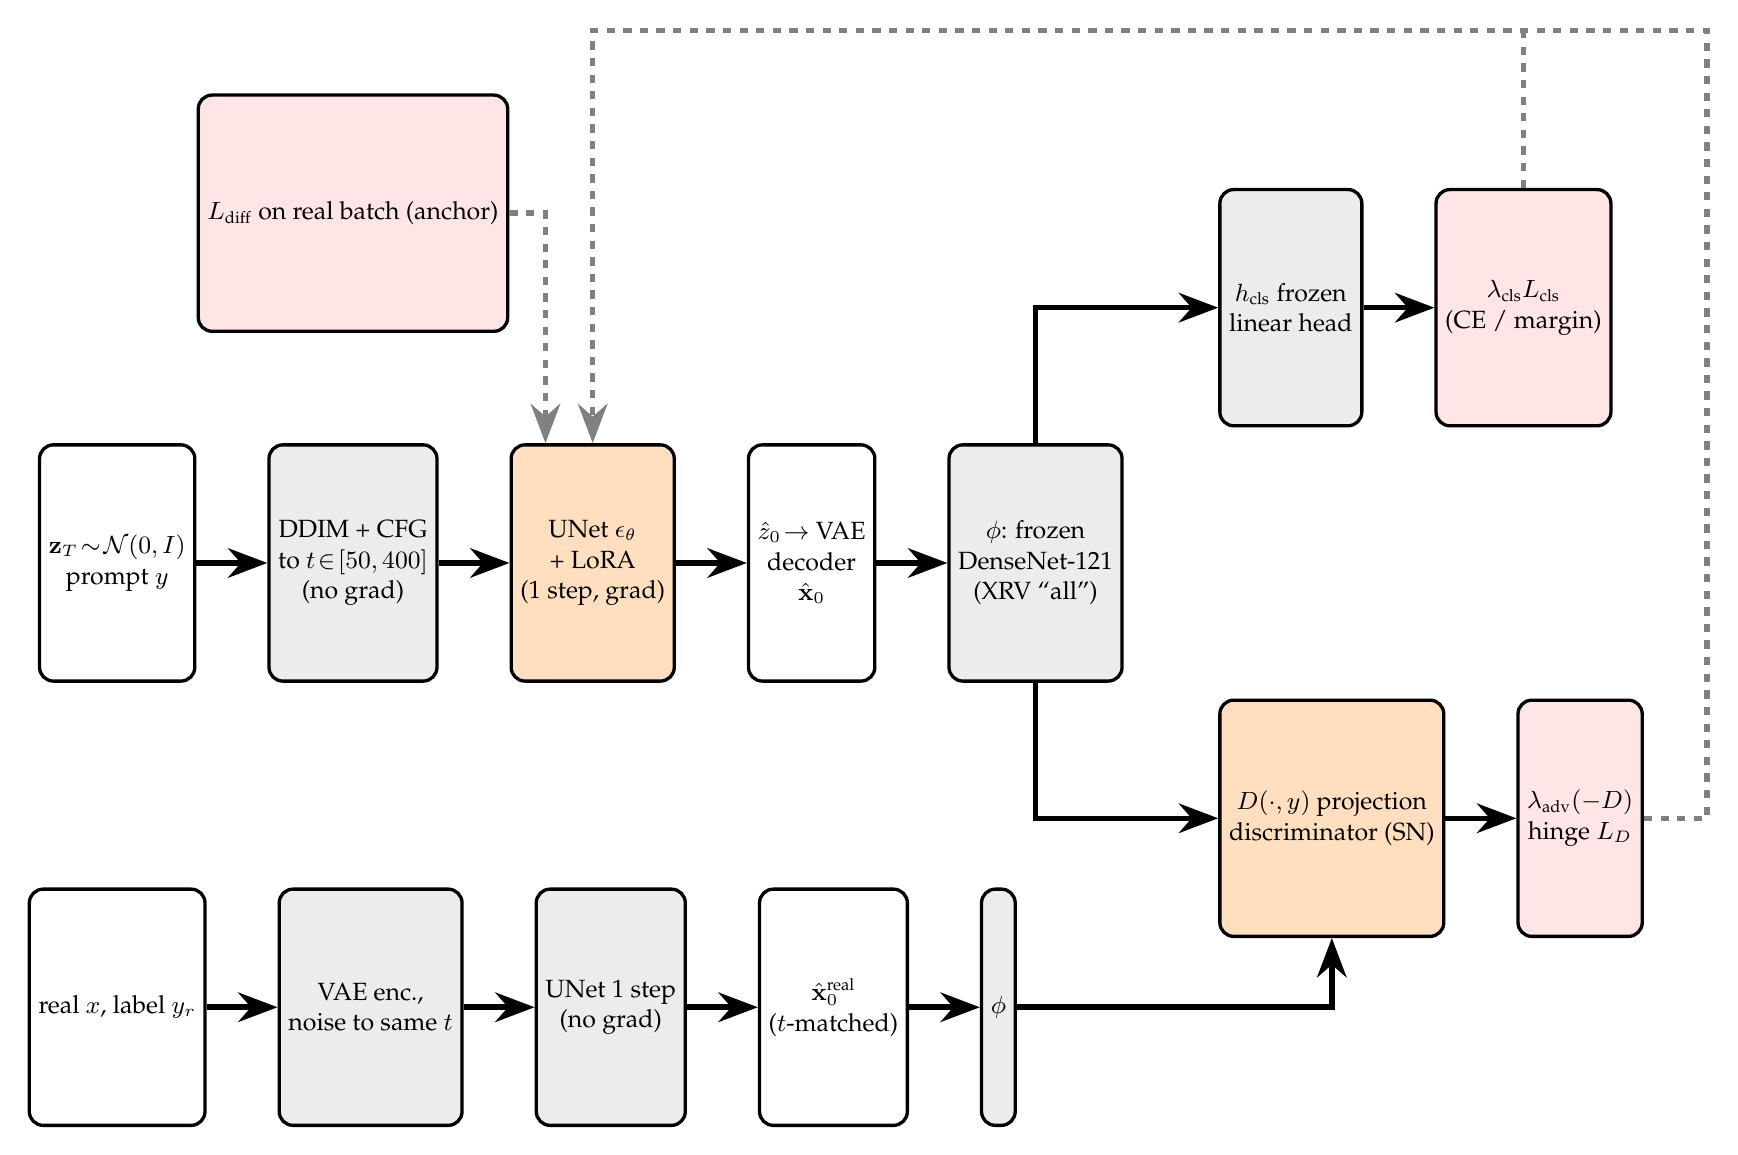
\begin{tikzpicture}[
  node distance=8mm and 9mm,
  b/.style={draw, very thick, rounded corners=5pt, align=center, font=\small, minimum height=3cm, fill=#1},
  b/.default=white,
  fr/.style={b=gray!15},
  tr/.style={b=orange!25},
  arr/.style={-{Stealth[length=5mm]}, line width=2pt},
  ng/.style={-{Stealth[length=5mm]}, line width=2pt, dashed, gray}]
\node[b] (noise) {$\z_{T}\!\sim\!\mathcal N(0,I)$\\prompt $y$};
\node[fr, right=of noise] (ddim) {DDIM + CFG\\to $t\!\in\![50,400]$\\(no grad)};
\node[tr, right=of ddim] (unet) {UNet $\epsilon_\theta$\\+ LoRA\\(1 step, grad)};
\node[b, right=of unet] (x0) {$\hat z_0\!\to$ VAE\\decoder\\$\hx$};
\node[fr, right=of x0] (phi) {$\phi$: frozen\\DenseNet-121\\(XRV ``all'')};
\node[fr, above right=2mm and 12mm of phi] (hcls) {$h_{\text{cls}}$ frozen\\linear head};
\node[tr, below right=2mm and 12mm of phi] (D) {$D(\cdot,y)$ projection\\discriminator (SN)};
\node[b=red!10, right=of hcls] (lcls) {$\lambda_{\text{cls}}L_{\text{cls}}$\\(CE / margin)};
\node[b=red!10, right=of D] (ladv) {$\lambda_{\text{adv}}(-D)$\\hinge $L_D$};
\node[b, below=26mm of noise] (real) {real $x$, label $y_r$};
\node[fr, right=of real] (noisy) {VAE enc.,\\noise to same $t$};
\node[fr, right=of noisy] (unet2) {UNet 1 step\\(no grad)};
\node[b, right=of unet2] (x0r) {$\hx^{\text{real}}$\\($t$-matched)};
\node[fr, right=of x0r] (phi2) {$\phi$};
\node[b=red!10, above=14mm of ddim] (ldiff) {$L_{\text{diff}}$ on real batch (anchor)};
\draw[arr] (noise)--(ddim); \draw[arr] (ddim)--(unet); \draw[arr] (unet)--(x0); \draw[arr] (x0)--(phi);
\draw[arr] (phi)|-(hcls); \draw[arr] (phi)|-(D); \draw[arr] (hcls)--(lcls); \draw[arr] (D)--(ladv);
\draw[arr] (real)--(noisy); \draw[arr] (noisy)--(unet2); \draw[arr] (unet2)--(x0r); \draw[arr] (x0r)--(phi2);
\draw[arr] (phi2)-|(D);
\coordinate (topy) at ($(ldiff.north)+(0,8mm)$);
\draw[ng] (ldiff.east)-|([xshift=-6mm]unet.north);
\draw[ng] (ladv.east)--++(8mm,0) |- (topy -| unet.north) -- (unet.north);
\draw[line width=2pt,dashed,gray] (lcls.north) -- (topy -| lcls.north);
\end{tikzpicture}}
\captionof{figure}{\color{Blue} Overall architecture. Orange = trainable, grey = frozen; dashed = gradients into the LoRA.}
\label{Arch}
\end{center}
\textbf{Generator objective} (one-step estimate $\hx$~[3,4]):
\[
L_G = L_{\text{diff}} \;+\; \lambda_{\text{cls}}\,L_{\text{cls}}\big(h_{\text{cls}}(\phi(\hx)),\,y\big) \;-\; \lambda_{\text{adv}}\,D\big(\phi(\hx),\,y\big)
\]
\begin{itemize}
	\item \textbf{Margin loss (ours):} $L_{\text{cls}}=\max(0,\, m_y-[s_y-\max_{k\neq y}s_k])$, $m_y$ = median margin of \emph{real} class-$y$ images; bounded, so not hackable.
	\item \textbf{Discriminator:} spectral-norm projection head~[5] on frozen features (ADD-style~[6]), hinge loss, real images noised to the same $t$.
	\item \textbf{Held-out judges:} finding = probe on XRV \texttt{mimic\_ch}~[7]; defect = PSPNet anatomy check fails or Mahalanobis OOD; KID.
\end{itemize}

%----------------------------------------------------------------------------------------
%	Dataset Details
%----------------------------------------------------------------------------------------
\section*{Dataset Details}
\textbf{CheXpert-v1.0-small}~[8] (224k CXRs, 65k patients, 14 labels); frontal, single-label, no uncertain labels, patient-disjoint.
\begin{center}
\resizebox{\linewidth}{!}{%
\begin{tabular}{lll}
\toprule
\textbf{Split} & \textbf{Images} & \textbf{Used for}\\
\midrule
Diffusion training & 4{,}401 (6 classes) & LoRA fine-tuning; real reference for $D$\\
\quad per class & \multicolumn{2}{l}{Fr 1{,}327; EC 978; NF 750; LL 732; Pn 373; PO 241}\\
Classifier training & 16{,}624 (14 cl.; 10\% val) & DenseNet-121, heads, judges; val = epoch choice\\
Test & 700 (50 per class) & final scores only\\
Synthetic / generator & 2{,}173 & 500 each EC, LL, Pn, PO; 173 Fracture\\
\bottomrule
\end{tabular}}
\captionof{table}{\color{Blue} Data splits.}
\end{center}

%----------------------------------------------------------------------------------------
%	Novelty Assessment
%----------------------------------------------------------------------------------------
\section*{Novelty Assessment}
\begin{itemize}
	\item \textbf{CE signal in LoRA fine-tuning} vs.\ P-Rajiv and a \emph{control} run (same extra steps, no new loss).
	\item \textbf{Adversarial ``comparable to real'' loss}, alone and with CE / margin; \textbf{multi-scale $D$} ablation.
	\item \textbf{Per-pathology} finding / defect rates for 10 generators, incl.\ DA-Fusion img2img~[9].
	\item \textbf{DenseNet with vs.\ without synthetic data} on the same real test set, plus a \emph{recipe}: real-count class weights, synthetic weight 0.5, last 3 epochs real-only.
\end{itemize}

%----------------------------------------------------------------------------------------
%	Results
%----------------------------------------------------------------------------------------
\section*{Results}
\begin{center}
\resizebox{\linewidth}{!}{%
\begin{tabular}{lccccc}
\toprule
 & \multicolumn{3}{c}{\textbf{Generation (held-out judges)}} & \multicolumn{2}{c}{\textbf{Downstream macro-F1}}\\
\textbf{Generator} & \textbf{Req.\ finding} $\uparrow$ & \textbf{Defects} $\downarrow$ & \textbf{KID}$\times10^3\downarrow$ & \textbf{plain} & \textbf{[recipe]}\\
\midrule
Real only (no synthetic) & 29.7\%$^\ast$ & -- & -- & \multicolumn{2}{c}{\textbf{0.285$\pm$0.012}}\\
P-Rajiv LoRA (baseline) & 15.7\% & 32.7\% & 12.8 & 0.256 & --\\
Control (more training) & 23.6\% & 51.8\% & 10.3 & 0.275 & --\\
CE only & 35.3\% & \textcolor{red}{78.5\%} & 29.9 & 0.258 & --\\
Adversarial only & 25.9\% & 9.8\% & 2.9 & 0.270 & --\\
CE + adversarial & 45.9\% & 24.6\% & 8.2 & 0.269 & \textbf{0.283}\\
\textbf{Margin + adversarial (ours)} & \textbf{51.2\%} & 18.2\% & 7.8 & 0.278 & 0.279\\
Margin + adv, multi-scale $D$ & 43.8\% & 16.5\% & 8.7 & 0.264 & 0.281\\
DA-Fusion img2img (from real) & 39.4\% & 10.4\% & 3.0 & 0.253 & 0.279$^\dagger$\\
\bottomrule
\end{tabular}}
\captionof{table}{\color{Blue} Mean over 5 target pathologies; downstream = DenseNet-121, 3 seeds, 700 real test images. $^\ast$probe on real images. $^\dagger$+ filter.}
\label{table}
\end{center}
\columnbreak
Table~\ref{table}: the combined losses \textbf{triple} the requested-finding rate and cut defects; CE alone \textbf{reward-hacks}. Downstream, the original augmentation \emph{hurts} (0.256); new generators + recipe reach \textbf{parity} (0.283 vs.\ 0.285, within seed noise).

\begin{center}
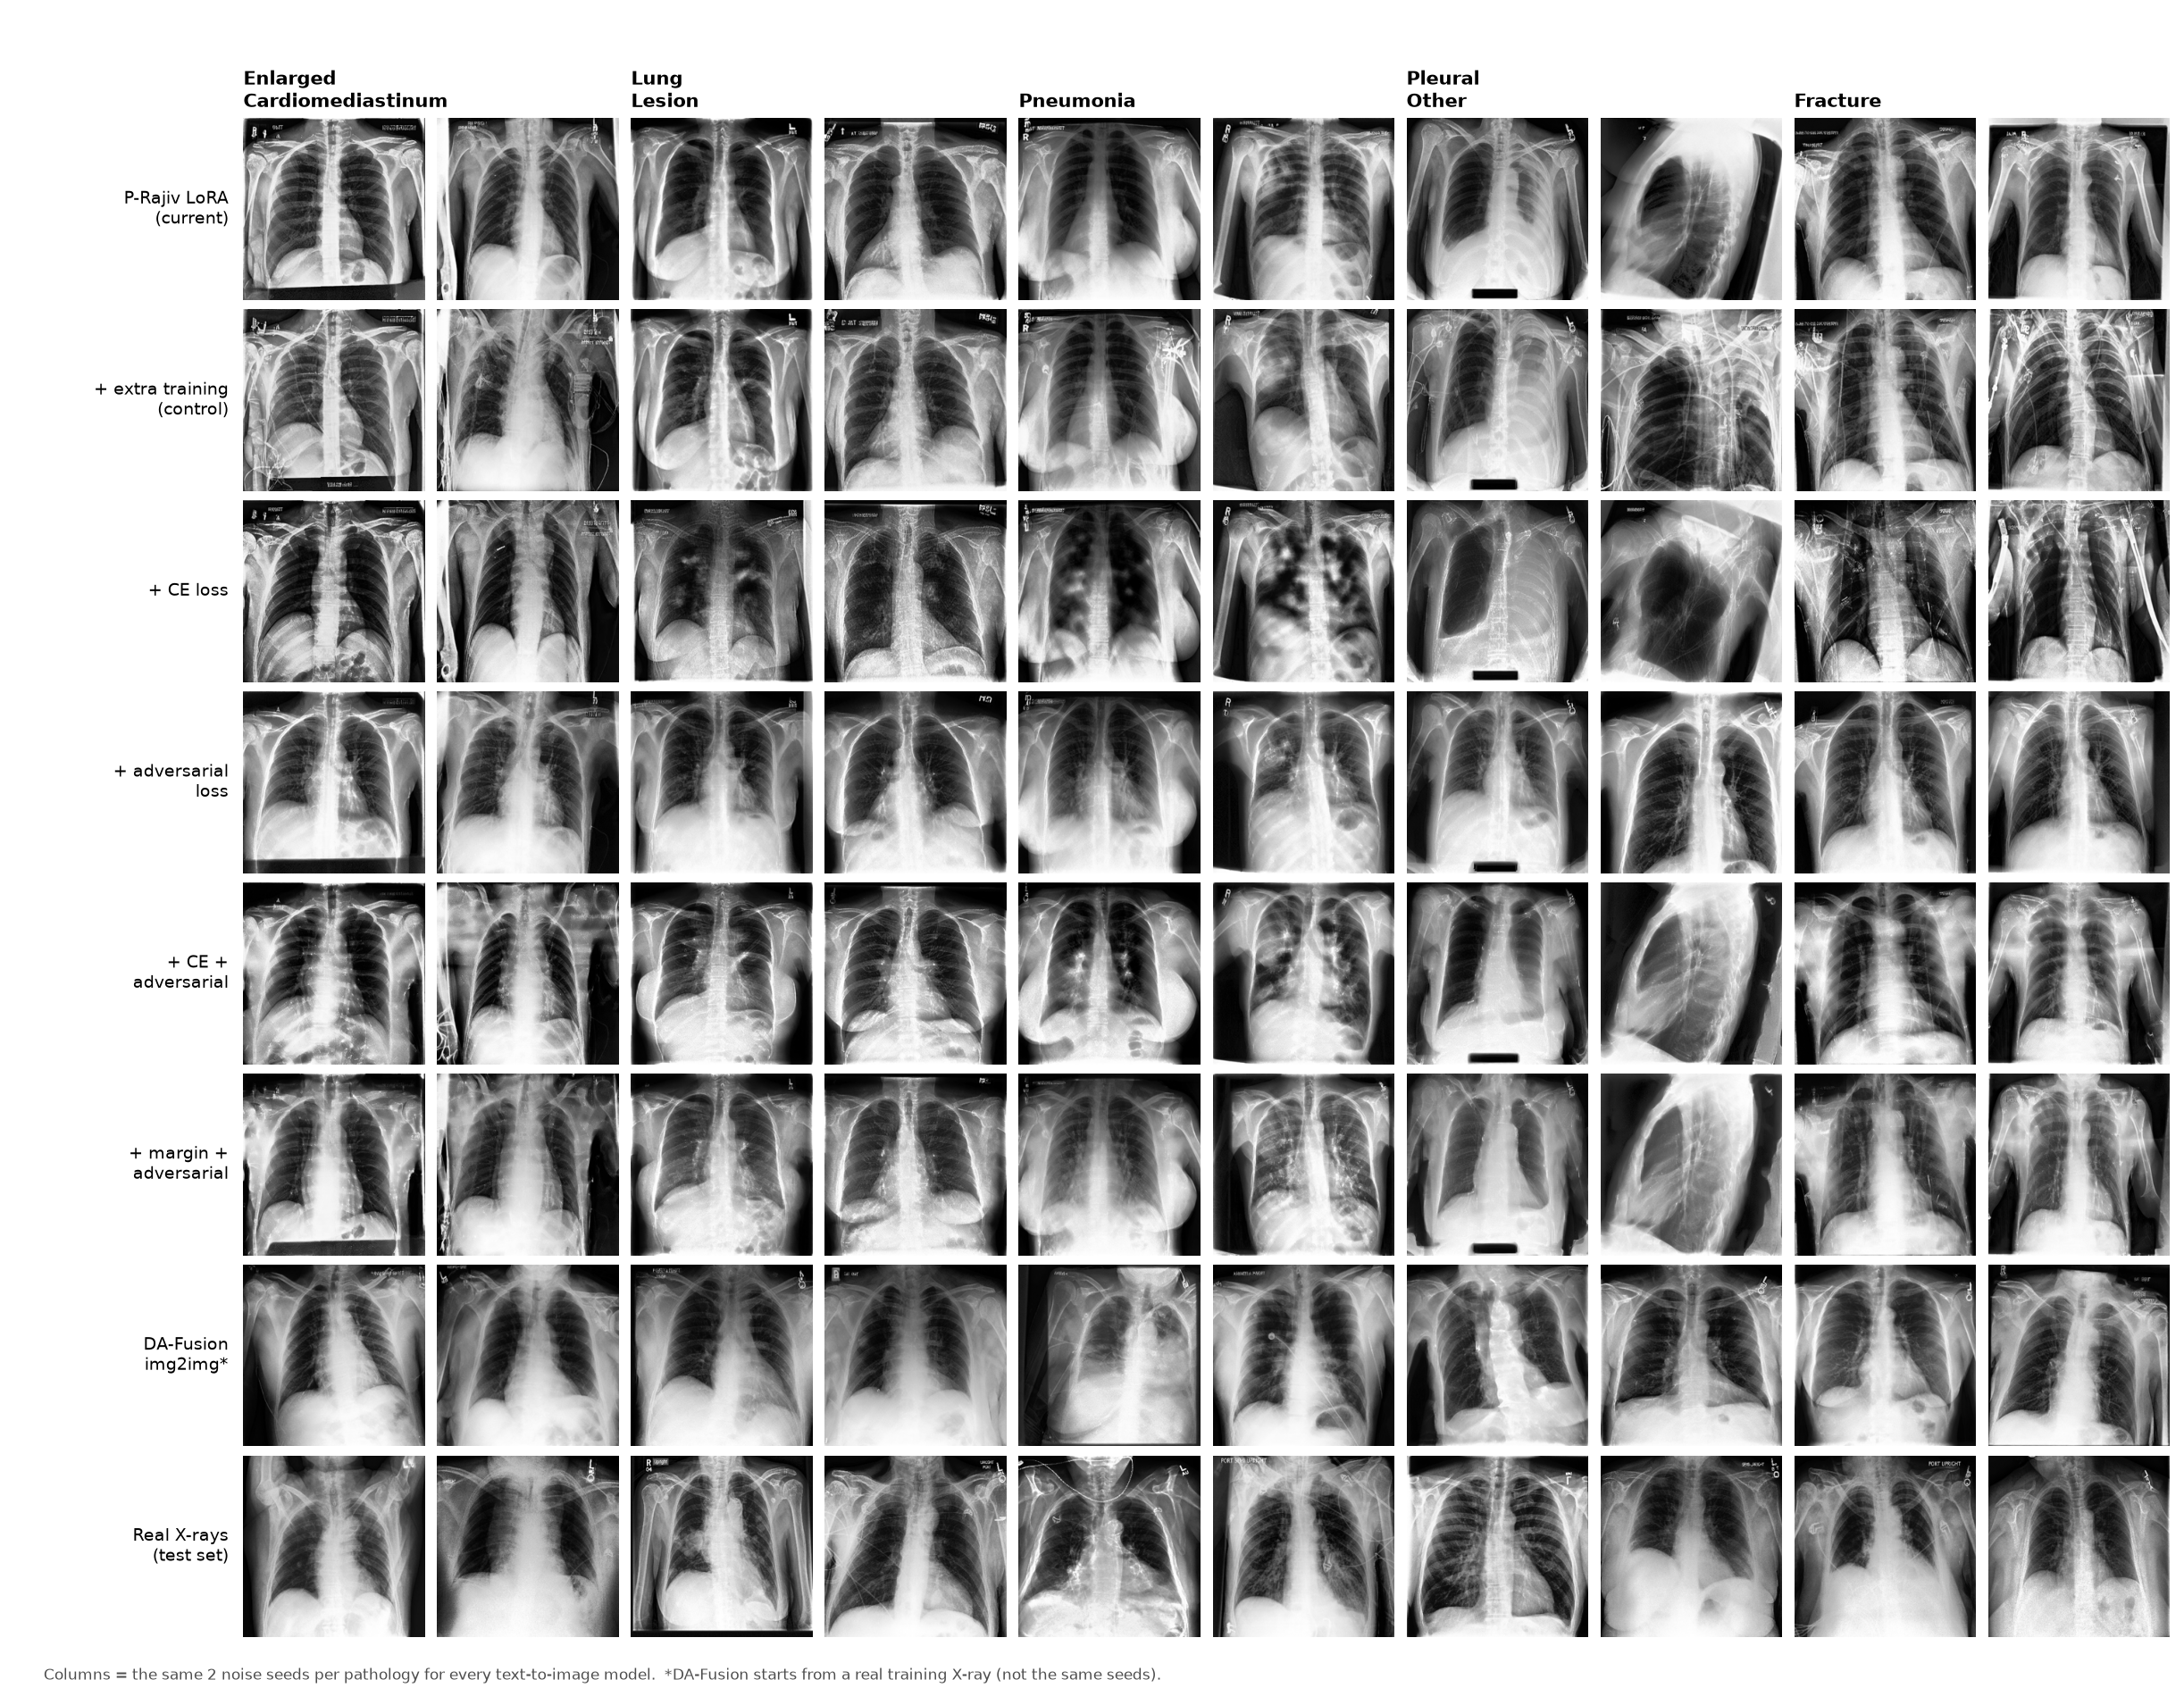
\includegraphics[width=0.58\linewidth]{fig_samples_same_seeds.png}
\captionof{figure}{\color{Blue} Same noise seeds through every generator. CE-only gives blotchy ``cotton-wool'' artefacts; adding the adversarial term restores anatomy.}
\end{center}

\begin{center}
\resizebox{\linewidth}{!}{%
\begin{tabular}{lccccc}
\toprule
\textbf{Finding / Defect (\%)} & \textbf{Enl.\ Cardiomed.} & \textbf{Lung Lesion} & \textbf{Pneumonia} & \textbf{Pleural Other} & \textbf{Fracture}\\
\midrule
P-Rajiv (baseline) & 12 / 33 & 6 / 31 & 14 / 29 & 29 / 34 & 18 / 35\\
CE only & 33 / \textcolor{red}{77} & 32 / \textcolor{red}{63} & 21 / \textcolor{red}{77} & 61 / \textcolor{red}{83} & 30 / \textcolor{red}{93}\\
Adversarial only & 44 / 9 & 6 / 10 & 18 / 11 & 28 / 10 & 34 / 9\\
CE + adversarial & \textbf{76} / 33 & \textbf{44} / 13 & 11 / 34 & \textbf{67} / 29 & 31 / 15\\
Margin + adv (ours) & 63 / 20 & 24 / 13 & \textbf{63} / 22 & 61 / 19 & 44 / 17\\
Margin + adv, multi-scale $D$ & 67 / 18 & 30 / 14 & 42 / 20 & 27 / 11 & \textbf{53} / 20\\
DA-Fusion img2img & 61 / 11 & 27 / 8 & 29 / 10 & 45 / 10 & 36 / 13\\
\bottomrule
\end{tabular}}
\captionof{table}{\color{Blue} Per-pathology requested-finding / structural-defect rate (held-out judges).}
\end{center}

\begin{center}
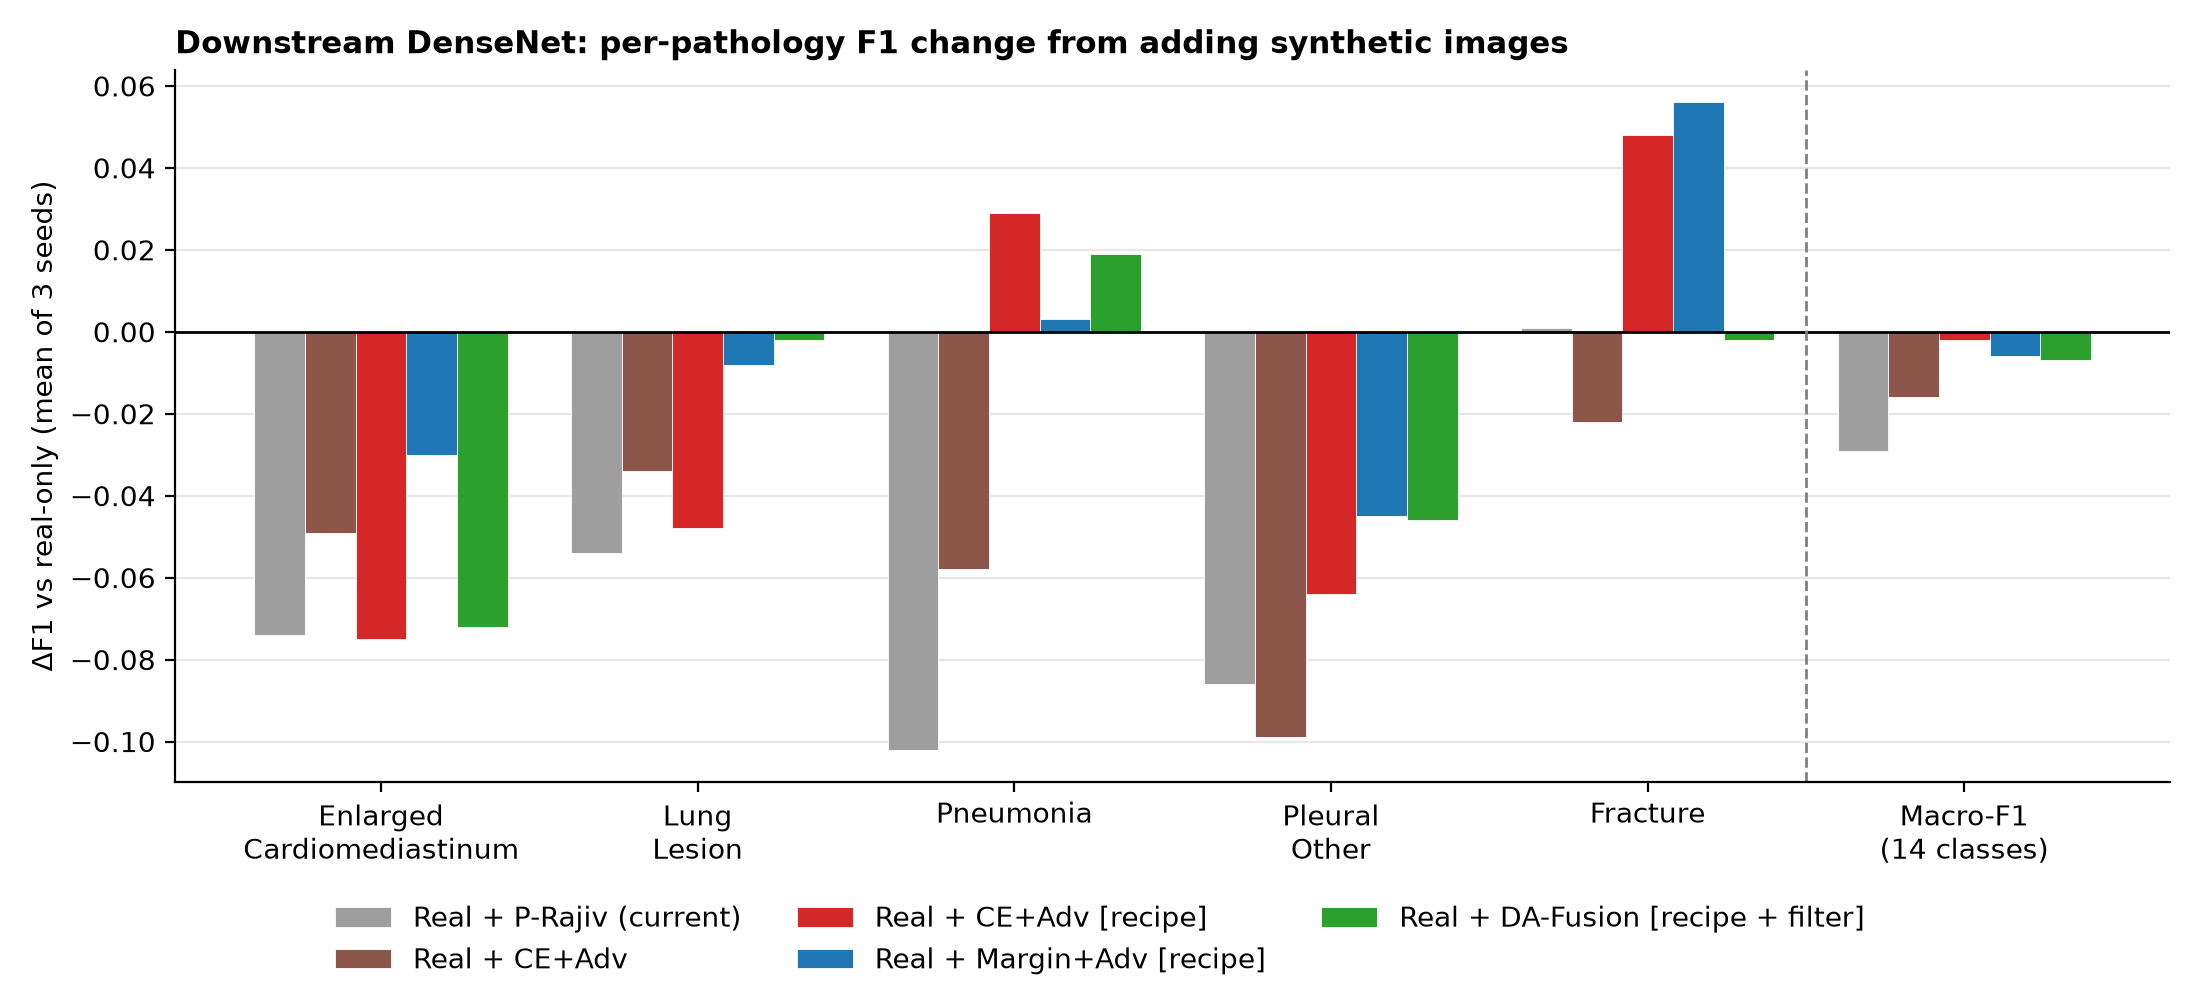
\includegraphics[width=0.78\linewidth]{fig_downstream_delta_key.png}
\captionof{figure}{\color{Blue} Per-pathology change in test F1 vs.\ real-only. Fracture improves (+0.05); Pleural Other is hurt except with the multi-scale $D$.}
\end{center}

\textbf{Why real + synthetic does not beat real-only here} --- consistent with the literature:
\begin{itemize}
	\item \textbf{Full data, in-distribution test:} gains are reported mainly with scarce real data~[2,10,11] or under distribution shift~[12]; we have 241--1{,}327 real images per class and a CheXpert test set.
	\item \textbf{No new information:} the generator learns from the same CheXpert images and labels; real data remains superior in this regime~[13,14].
	\item \textbf{Image metrics $\neq$ usefulness}~[14]: CE+Adv shows Enl.\ Cardiomed.\ in 76\% of images, yet its F1 drops 0.311$\to$0.236. Label noise (probe: 29.7\% on real) and 50 test images/class limit what can be resolved ($<$0.03 F1).
\end{itemize}

%----------------------------------------------------------------------------------------
%	CONCLUSIONS
%----------------------------------------------------------------------------------------
\section*{Conclusion}
\begin{itemize}
	\item Classifier + adversarial losses make a LoRA CXR generator follow the prompt: \textbf{15.7\%$\to$51.2\%} requested finding, \textbf{32.7\%$\to$18.2\%} defects, KID 12.8$\to$7.8.
	\item A classifier signal alone is reward-hackable; a bounded \textbf{margin} loss plus an adversarial regulariser controls it.
	\item Better images turn a harmful augmentation into \textbf{parity} with real-only training, with gains on Fracture, but not an overall improvement.
	\item Next: low-data and shifted-test-set experiments, where synthetic data is expected to help; rewarding downstream usefulness directly.
\end{itemize}

%----------------------------------------------------------------------------------------
%	References
%----------------------------------------------------------------------------------------
\section*{References}
{\scriptsize\setlength{\columnseprule}{0pt}\setlength{\columnsep}{40pt}
\begin{multicols}{2}
\begin{enumerate}[label={[\arabic*]}, leftmargin=*, itemsep=0pt, topsep=0pt]
\item Rombach, R., et al.: High-resolution image synthesis with latent diffusion models. CVPR (2022)
\item Chambon, P., et al.: RoentGen: Vision-language foundation model for chest X-ray generation. arXiv:2211.12737 (2022)
\item Xu, J., et al.: ImageReward: Learning and evaluating human preferences for text-to-image generation. NeurIPS (2023)
\item Clark, K., et al.: Directly fine-tuning diffusion models on differentiable rewards. ICLR (2024)
\item Miyato, T., Koyama, M.: cGANs with projection discriminator. ICLR (2018)
\item Sauer, A., et al.: Adversarial diffusion distillation. arXiv:2311.17042 (2023)
\item Cohen, J.P., et al.: TorchXRayVision: A library of chest X-ray datasets and models. MIDL (2022)
\item Irvin, J., et al.: CheXpert: A large chest radiograph dataset with uncertainty labels and expert comparison. AAAI (2019)
\item Trabucco, B., et al.: Effective data augmentation with diffusion models. ICLR (2024)
\item He, R., et al.: Is synthetic data from generative models ready for image recognition? ICLR (2023)
\item Prakash, E., et al.: Evaluating and improving the effectiveness of synthetic chest X-rays for medical image analysis. ICCVW (2025)
\item Ktena, I., et al.: Generative models improve fairness of medical classifiers under distribution shifts. Nature Medicine 30, 1166--1173 (2024)
\item Khosravi, B., et al.: Synthetically enhanced: Unveiling synthetic data's potential in medical imaging research. eBioMedicine (2024)
\item Ravuri, S., Vinyals, O.: Classification accuracy score for conditional generative models. NeurIPS (2019)
\end{enumerate}
\end{multicols}}

%----------------------------------------------------------------------------------------
%	ACKNOWLEDGEMENTS
%----------------------------------------------------------------------------------------
\section*{Acknowledgments}
\small \textnormal{We thank \textbf{the IE643 instructor and TAs} for the review feedback, and the Stanford ML Group for CheXpert.}

\section*{Github Link and Demo Video Link}
\vspace{-0.5cm}
\begin{center}
		\begin{minipage}{0.4\linewidth}
			\centering
			\textbf{Github Repository}\\[1ex]
			\fbox{\parbox[c][0.32\linewidth][c]{0.32\linewidth}{\centering\todo{QR code\\to be added}}}
		\end{minipage}\hfill
		\begin{minipage}{0.4\linewidth}
			\centering
			\textbf{Demo Video Link}\\[1ex]
			\fbox{\parbox[c][0.32\linewidth][c]{0.32\linewidth}{\centering\todo{QR code\\to be added}}}
		\end{minipage}
\end{center}

\end{multicols}
\vspace{0.5cm}
\end{framed}
\end{minipage}
\end{document}
